\subsection{Drag \& drop}

\subsection{Tworzenie własnych komponentów}

Jedną z najciekawszych możliwości nowoczesnych technologii informatycznych jest możliwość definiowania
własnych komponentów wizualnych. Kiedy nie było jeszcze technologii .NET własne komponenty można było
tworzyć w technologii COM, używając do tego Visual Basica lub C++. 

Możliwości .NET jeszcze bardziej ułatwiają cały ten proces. Tak naprawdę wystarczy utworzyć klasę
dziedziczącą z {\bf UserControl} i już może ona funkcjonować jako komponent wizualny. Taki własny
komponent może na przykład składać się z dowolnej ilości już istniejących komponentów i automatyzować
pewne zależności między nimi, może też tworzyć całkowicie nowe możliwości interfejsowe.

Do czego może przydawać się możliwość tworzenia własnych komponentów? 

Wyobraźmy sobie na przykład, że
standardowy komponent {\bf ComboBox} chcielibyśmy wyposażyć w automatyczne dopasowywanie elementu na liście
do tekstu wpisywanego przez użytkownika. Zwykły ComboBox tego nie potrafi, ale można utworzyć własny
komponent i dodać reakcje na odpowiednie zdarzenia, by uzyskać porządaną funkcjonalność. Można taki problem
rozwiązać bez tworzenia nowego komponentu, tyle że gdyby chcieć użyć takiego ComboBoxa więcej niż raz,
utworzenie jednego komponentu wielokrotnego użycia, po prostu ogromnie upraszcza życie programisty.

Wyobraźmy sobie również, że chcielibyśmy mieć zupełnie nowy komponent wizualny, siatkę, z możliwością
dodawania wierszy i kolumn i to taką, żeby każda komórka mogła mieć inny kolor, czcionkę wyrównanie czy
orientację tekstu. Takiego komponentu standardowo w bibliotece komponentów .NET nie ma.
Możnaby jednak utworzyć własny komponent, dodać mu jakieś struktury danych do przechowywania danych,
dodać jakieś propercje, metody i zdarzenia, tak aby można było sterować takim komponentem z poziomu kodu
konkretnego okna, w którym byłby on osadzony, a następnie przeciążyć całkowicie metodę {\bf OnPaint}, dzięki
czemu wizualna zawartość komponentu mogłaby być tworzona całkowicie dowolnie, bez żadnego związku z już
istniejącymi komponentami.

\subsubsection{Najprostszy komponent}

Zaczniemy od bardzo prostego przykładu komponentu, który będzie tylko
wypisywał tekst w swoim obszarze. Komponent taki jset oknem leżącym gdzieś w jakimś innym oknie.
Wewnątrz kodu może więc dowiedzieć się jakie są jego bieżące rozmiary za pomocą propercji
{\bf Width} i {\bf Height}. Również propercje takie jak {\bf Font}, {\bf Text}, {\bf BackColor} czy
{\bf ForeColor} są, jako dziedziczone z klasy {\bf UserControl}, dostępne dla klienta komponentu.

Klient komponentu (czyli kod, który korzysta z tego komponentu) traktuje więc nowo zaprojektowany komponent
jak każdy inny - może ustalać rozmiary komponentu, jego kotwicowanie czy dokowanie oraz używać 
wszystkich potrzebnnych propercji, zdarzeń i metod (tak prosty komponent nie ma żadnych sensownych
składowych poza tymi dziedziczonymi z {\bf UserControl}).

W środowisku wizualnym tak zaprojektowany komponent po umieszczeniu w bibliotece obiektowej
(takie jest ograniczenie na przykład VisualStudio) mógłby być umieszczony na przyborniku z komponentami i
umieszczany na oknach jak każdy inny komponent z przybornika!

\begin{figure}
\begin{center}
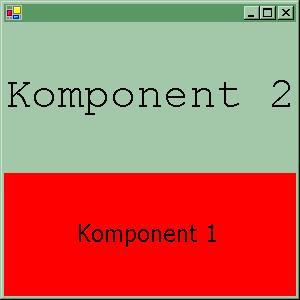
\includegraphics[width=0.50\textwidth]{./pic/swf06}
\caption{Najprostszy komponent}
\end{center}
\end{figure}

\begin{scriptsize}
\begin{verbatim}
/* Wiktor Zychla, 2003 */
using System;
using System.Drawing;
using System.Windows.Forms;

namespace Example
{
  public class CKomponent : UserControl
  {
    public CKomponent() {}

    protected override void OnPaint( PaintEventArgs e )
    {
      StringFormat sf  = new StringFormat();
      sf.Alignment     = StringAlignment.Center;
      sf.LineAlignment = StringAlignment.Center;

      e.Graphics.Clear( this.BackColor );
      e.Graphics.DrawString( this.Text, this.Font, Brushes.Black, 
                             this.Width / 2, this.Height / 2, sf );
    }

    protected override void OnResize( EventArgs e )
    {
      Invalidate();
    }
  }

  public class CMainForm : Form
  {  
    CKomponent ck1, ck2;

    public CMainForm() 
    {
      ck1      = new CKomponent();
      ck1.Text = "Komponent 1";
      ck1.BackColor = Color.Red;
      ck1.Font = new Font( "Tahoma", 18 );
      ck1.Size = new Size( 50, 50 );
      ck1.Dock = DockStyle.Fill;

      ck2      = new CKomponent();
      ck2.Text = "Komponent 2";
      ck2.Font = new Font( "Courier", 32 );
      ck2.Dock = DockStyle.Top;

      this.Controls.AddRange( new Control[] { ck1, ck2 } );
    }

    public static void Main()
    {    
      Application.Run( new CMainForm() );
    }
  }
}
\end{verbatim}
\end{scriptsize}

\subsubsection{Komponent złożony}

Komponent może zawierać w sobie dowolną ilość innych komponentów i wewnątrz swojego kodu
przechwytywać ich zdarzenia.

\begin{scriptsize}
\begin{verbatim}
/* Wiktor Zychla, 2003 */
using System;
using System.Drawing;
using System.Windows.Forms;

namespace Example
{
  public class CKomponent : UserControl
  {
    Button b1, b2;

    public CKomponent() 
    {
      b1      = new Button();
      b1.Text = "1";
      b1.Dock = DockStyle.Fill;
      b1.Click += new EventHandler( bt_Click );

      b2      = new Button();
      b2.Text = "2";
      b2.Size = new Size( 40, 40 );
      b2.Dock = DockStyle.Right;
      b2.Click += new EventHandler( bt_Click );

      this.Controls.AddRange( new Control[] { b1, b2 } );
    }

    public void bt_Click( object sender, EventArgs e )
    {
      MessageBox.Show( ((Control)sender).Text );
    } 
  }

  public class CMainForm : Form
  {  
    CKomponent ck1, ck2;

    public CMainForm() 
    {
      ck1      = new CKomponent();
      ck1.Text = "Komponent 1";
      ck1.BackColor = Color.Red;
      ck1.Font = new Font( "Tahoma", 8 );
      ck1.Size = new Size( 50, 50 );
      ck1.Dock = DockStyle.Fill;

      ck2      = new CKomponent();
      ck2.Text = "Komponent 2";
      ck2.Font = new Font( "Courier", 12 );
      ck2.Dock = DockStyle.Top;

      this.Controls.AddRange( new Control[] { ck1, ck2 } );
    }

    public static void Main()
    {    
      Application.Run( new CMainForm() );
    }
  }
}
\end{verbatim}
\end{scriptsize}

\subsubsection{Definiowanie własnych zdarzeń}

Zestaw zdarzeń udostępnianych przez komponenty również może być rozbudowany. Wyobraźmy sobie, że
chcielibyśmy mieć komponent, który zawierałby {\bf ComboBox} i mały przycisk z napisem "+" z boku.
Chcielibyśmy, aby użytkownik mógł użyć tego przycisku do dodawania nowych elementów do ComboBoxa.
Z punktu widzenia logiki tego komponentu zdarzenie oznaczające chęć dodania nowego elementu mogłoby
jednak pojawiać się również wtedy, kiedy użytkownik wpisałby w pole tekstowe {\bf ComboBoxa} jakiś tekst spoza
tekstów dostępnych na liście. To już aż dwa przypadki, kiedy takie zdarzenie mogłoby się pojawić.

Możemy więc zaprojektować nowe zdarzenie. Nazwiemy je {\bf AddNewText}. Być może w toku prac
okazałobysię, że zdarzenie takie powinno mieć jakieś dodatkowe parametry. Zaprojektowalibyśmy wtedy
nową klasę, {\bf AddNewTextEventArgs} i zmodyfikowalibyśmy deklarację zdarzenia. Należałoby jedynie
pamiętać o zachowaniu konwencji: odpowiedni delegat powinien mieć dwa parametry, z czego pierwszy
powinien wskazywać na źródło zdarzenia, drugi powinien dziedziczyć z klasy {\bf EventArgs},
rozszerzając ją o dodatkowe parametry zdarzenia.

Zauważmy, że kod klienta korzysta z tego zdarzenia tak samo jak z każdego zdarzenia. Z punktu widzenia
kodu nie ma różnicy między naszym nowym zdarzeniem, a już istniejącymi zdarzeniami.

\begin{scriptsize}
\begin{verbatim}
/* Wiktor Zychla, 2003 */
using System;
using System.Drawing;
using System.Windows.Forms;

namespace Example
{  
  public class CComboBox : UserControl
  {
    ComboBox cb;
    Button   bt;

    // własne zdarzenie definiowane przez komponent
    public event EventHandler AddNewText;

    public CComboBox() 
    {
      cb      = new ComboBox(); 
      cb.Dock = DockStyle.Fill;
      
      bt      = new Button();
      bt.FlatStyle = FlatStyle.Popup;
      bt.Text = "+";
      bt.Dock = DockStyle.Right; 
      bt.Click += new EventHandler( bt_Click );

      this.Controls.AddRange( new Control[] { cb, bt } );
    }

    protected override void OnResize( EventArgs e )
    {
      bt.Size = new Size( this.Height, this.Height );           
    }    

    // przechwyć klik w przycisk i na zewnątrz wystaw jako AddNewText
    void bt_Click( object sender, EventArgs e )
    {
      // sprawdź czy są jacyś słuchacze     
      if ( AddNewText != null )
        AddNewText( this, new EventArgs() );
    }
  }

  public class CMainForm : Form
  {  
    CComboBox cb1;

    public CMainForm() 
    {
      cb1      = new CComboBox();
      cb1.Size = new Size( 150, 20 );

      cb1.AddNewText += new EventHandler( cb_AddNewText );

      this.Controls.Add( cb1 );
    }

    void cb_AddNewText( object sender, EventArgs e )
    {
      MessageBox.Show( "Zgłoszono zdarzenie AddNewText!" );
    }

    public static void Main()
    {    
      Application.Run( new CMainForm() );
    }
  }
}
\end{verbatim}
\end{scriptsize}

\subsection{Typowe okna dialogowe}

\subsubsection{Okna wyboru plików}

Standardowo, programista ma do dyspozycji okno wyboru pliku do otwarcia i zamknięcia
({\bf OpenFileDialog} i {\bf SaveFileSialog}). Oba działają
bardzo podobnie - po ustaleniu właściwości należy wywołać metodę do pokazania okna i
przechwycić rezultat, wskazujący na to czy przypadkiem użytkownik nie anulował okna. 
Lista wybranych plików dostępna jest dzięki propercji {\bf FileName[s]}.

\begin{scriptsize}
\begin{verbatim}
/* Wiktor Zychla, 2003 */
using System;
using System.Drawing;
using System.Windows.Forms;

namespace Example
{
  public class CMainForm : Form
  {  
    public CMainForm() 
    {
      OpenFileDialog of   = new OpenFileDialog();
      of.InitialDirectory = 
        Environment.GetFolderPath( Environment.SpecialFolder.ProgramFiles );
      of.Title            = "Wybierz plik do otwarcia...";
      of.Filter           = "Moje pliki (*.xyz)|*.xyz|"+
                            "Wszystkie pliki (*.*)|*.*";
      of.Multiselect      = true;

      DialogResult res = of.ShowDialog();
      if ( res == DialogResult.OK )
        foreach ( string fileName in of.FileNames )
          MessageBox.Show( "Wybrano plik " + fileName );
    }

    public static void Main()
    {    
      Application.Run( new CMainForm() );
    }
  }
}
\end{verbatim}
\end{scriptsize}

\subsubsection{Okno wyboru czcionki}

\begin{scriptsize}
\begin{verbatim}
/* Wiktor Zychla, 2003 */
using System;
using System.Drawing;
using System.Windows.Forms;

namespace Example
{
  public class CMainForm : Form
  {  
    public CMainForm() 
    {
      FontDialog fd    = new FontDialog();
      fd.ShowColor     = true;
      fd.ShowEffects   = true;

      DialogResult res = fd.ShowDialog();
      if ( res == DialogResult.OK )
        MessageBox.Show( "Wybrano czcionkę: " + fd.Font.ToString() );
    }

    public static void Main()
    {    
      Application.Run( new CMainForm() );
    }
  }
}
\end{verbatim}
\end{scriptsize}

\subsubsection{Okno wyboru koloru}

\begin{scriptsize}
\begin{verbatim}
/* Wiktor Zychla, 2003 */
using System;
using System.Drawing;
using System.Windows.Forms;

namespace Example
{
  public class CMainForm : Form
  {  
    public CMainForm() 
    {
      ColorDialog cd   = new ColorDialog();
      cd.AllowFullOpen = true;

      DialogResult res = cd.ShowDialog();
      if ( res == DialogResult.OK )
        MessageBox.Show( "Wybrano kolor: " + cd.Color.ToString() );
    }

    public static void Main()
    {    
      Application.Run( new CMainForm() );
    }
  }
}
\end{verbatim}
\end{scriptsize}
